\documentclass{article}
\usepackage[utf8]{inputenc}
\usepackage{amsthm}
\usepackage{amsmath}
\usepackage{amsfonts}
\usepackage{amssymb}
\usepackage{xcolor}
\usepackage{mathtools}
\usepackage{pgfplots}
\usepackage{wrapfig}    %https://www.overleaf.com/learn/latex/Wrapping_text_around_figures
\pgfplotsset{width=10cm,compat=1.9} %https://www.overleaf.com/learn/latex/Pgfplots_package#Reference_guide
\usepgfplotslibrary{fillbetween} %https://tex.stackexchange.com/questions/242311/filling-area-under-a-function
\usepackage{tikz}
\usetikzlibrary{shapes.geometric, arrows}   %https://www.overleaf.com/project/52205bbce77a8bec1415bf38
\usetikzlibrary{calc}   %https://tex.stackexchange.com/questions/71478/how-to-center-one-node-exactly-between-two-others-with-tikz


\begin{document}
	$T={I\times I}/{\{0,t\}\sim\{1,t\},\{t,0\}\sim\{t,1\}:\forall t\in[0,1]\}}$\\
	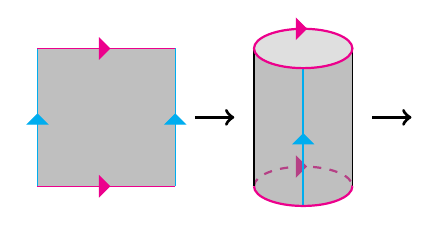
\begin{tikzpicture}[scale=.5, every node/.style={sloped,allow upside down}]
			%cuadrado (toro desarrollo)
			\fill[fill=gray,opacity=.5] (0,0) rectangle (3.5,3.5);
			\draw[cyan] (3.5,0) -- node {\tikz \draw[-triangle 90] (0,0) -- +(.1,0);} (3.5,3.5);
			\draw[cyan] (0,0) -- node {\tikz \draw[-triangle 90] (0,0) -- +(.1,0);} (0,3.5);
			\draw[magenta] (0,0) -- node {\tikz \draw[-triangle 90] (0,0) -- +(.1,0);} (3.5,0);
			\draw[magenta] (0,3.5) -- node {\tikz \draw[-triangle 90] (0,0) -- +(.1,0);} (3.5,3.5);
			
			\draw[very thick,->] (4,1.75) -- (5,1.75);
			
			%cilindro (toro semidesarrollado)
			\draw[magenta,thick,dashed] (5.5,0) arc (180:360:1.25 and -0.5) -- (8,0);
			\draw[magenta,-triangle 90] (6.75,.5) -- +(.1,0);
			\fill[gray,opacity=0.5] (5.5,3.5) -- (5.5,0) arc (180:360:1.25 and 0.5) -- (8,3.5) arc (0:180:1.25 and -0.5);
			\draw[] (5.5,3.5) -- (5.5,0);
			\draw[] (8,3.5) -- (8,0);
			\draw[cyan,thick] (6.75,-.5) -- node {\tikz \draw[-triangle 90] (0,0) -- +(.1,0);} (6.75,3);
			\filldraw[color=magenta,thick,fill=gray,fill opacity=.25] (6.75,3.5) ellipse (1.25 and 0.5);
			\draw[magenta,-triangle 90] (6.75,4) -- +(.1,0);
			\draw[magenta,thick] (5.5,0) arc (180:360:1.25 and 0.5) -- (8,0);
			
			\draw[very thick,->] (8.5,1.75) -- (9.5,1.75);
	\end{tikzpicture}
	$\vcenter{\hbox{
			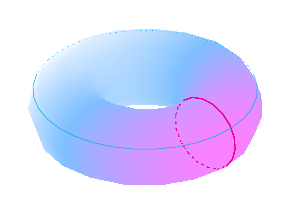
\begin{tikzpicture}[scale=.5]
					%toro
					\begin{axis}[
							hide axis,
							axis equal image,
							view={45}{32},
					%    zmin=-2.5,
					%    zmax=2.5,
					]
					
					\addplot3 [ %toro
							surf,
							shader     = interp,
							colormap/cool,
							opacity=.5,
					%    fill opacity=.2,
							draw,
							point meta = x,
							samples    = 10,    %20
							samples y  = 20,    %40
							z buffer   = sort,
							domain     = 0:360,
							y domain   = 0:360
					] (
							{(2+cos(x))*cos(y)},
							{(2+cos(x))*sin(y)},
							{sin(x)}
					);
					\addplot3 [ %anillo magenta (alante)
							mesh,
							color=magenta,
							opacity=1,
							loosely dotted,
							point meta = x,
							samples    = 10,
					%    samples y  = 1,
							z buffer   = sort,
							domain     = 135:315,
					%    y domain   = 5:5
					] (
							{(2+cos(x))*cos(5)},
							{(2+cos(x))*sin(5)},
							{sin(x)}
					);
					\addplot3 [ %anillo magenta (atras)
							mesh,
							opacity=1,
							draw=magenta,
							point meta = x,
							samples    = 10,
					%    samples y  = 1,
							z buffer   = sort,
							domain     = -45:135,
					%    y domain   = 5:5
					] (
							{(2+cos(x))*cos(5)},
							{(2+cos(x))*sin(5)},
							{sin(x)}
					);
					\addplot3 [ %anillo cian (alante)
							mesh,
							opacity=1,
							loosely dotted,
							color=cyan,
							point meta = x,
							samples    = 2,
							samples y  = 20,
							z buffer   = sort,
							domain     = 0:360,
							y domain   = 60:210
					] (
							{(2+cos(30))*cos(y)},
							{(2+cos(30))*sin(y)},
							{sin(30)}
					);
					\addplot3 [ %anillo cian (atras)
							mesh,
							opacity=1,
							color=cyan,
							point meta = x,
							samples    = 2,
							samples y  = 20,
							z buffer   = sort,
							domain     = 0:360,
							y domain   = -150:60
					] (
							{(2+cos(30))*cos(y)},
							{(2+cos(30))*sin(y)},
							{sin(30)}
					);
					\end{axis}
			\end{tikzpicture}
	}}$
						
						
						
\newpage

						
						
						
	$K={I\times I}/{\{s,0\}\sim\{s,1\},\{0,t\}\sim\{1,1-t\}:\forall s,t\in[0,1]\}}$\\            
	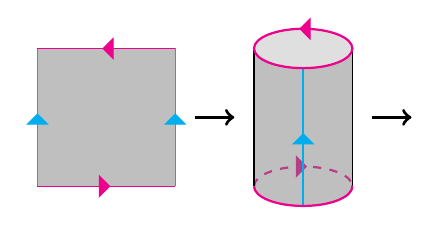
\begin{tikzpicture}[scale=.5, every node/.style={sloped,allow upside down}]
			%cuadrado (klein desarrollo)
			\fill[fill=gray,opacity=.5] (0,0) rectangle (3.5,3.5);
			\draw[cyan] (3.5,0) -- node {\tikz \draw[-triangle 90] (0,0) -- +(.1,0);} (3.5,3.5);
			\draw[cyan] (0,0) -- node {\tikz \draw[-triangle 90] (0,0) -- +(.1,0);} (0,3.5);
			\draw[magenta] (0,0) -- node {\tikz \draw[-triangle 90] (0,0) -- +(.1,0);} (3.5,0);
			\draw[magenta] (3.5,3.5) -- node {\tikz \draw[-triangle 90] (0,0) -- +(.1,0);} (0,3.5);
			
			\draw[very thick,->] (4,1.75) -- (5,1.75);
			
			%cilindro (klein semidesarrollado)
			\draw[magenta,thick,dashed] (5.5,0) arc (180:360:1.25 and -0.5) -- (8,0);
			\draw[magenta,-triangle 90] (6.75,.5) -- +(.1,0);
			\fill[gray,opacity=0.5] (5.5,3.5) -- (5.5,0) arc (180:360:1.25 and 0.5) -- (8,3.5) arc (0:180:1.25 and -0.5);
			\draw[] (5.5,3.5) -- (5.5,0);
			\draw[] (8,3.5) -- (8,0);
			\draw[cyan,thick] (6.75,-.5) -- node {\tikz \draw[-triangle 90] (0,0) -- +(.1,0);} (6.75,3);
			\filldraw[color=magenta,thick,fill=gray,fill opacity=.25] (6.75,3.5) ellipse (1.25 and 0.5);
			\draw[magenta,-triangle 90] (6.75,4) -- +(-.1,0);
			\draw[magenta,thick] (5.5,0) arc (180:360:1.25 and 0.5) -- (8,0);
			
			\draw[very thick,->] (8.5,1.75) -- (9.5,1.75);
	\end{tikzpicture}
	$\vcenter{\hbox{
	
			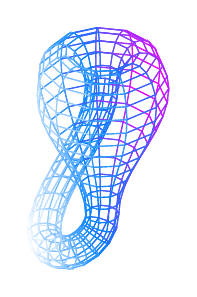
\begin{tikzpicture}[scale=1,very thin]
					%toro
					\begin{axis}[
							hide axis,
							axis equal image,
							view={30}{32+180},
							zmin=-2.5,
							zmax=12,
					]
					
					\addplot3 [ %brazo
							mesh,
							shader     = interp,
							colormap/cool,
					%    opacity=.5,
					%    fill opacity=.2,
							draw,
							point meta = x,
							samples    = 12,    %20
							samples y  = 10,    %40
							z buffer   = sort,
							domain     = 0:360,
							y domain   = 540:720
					] (
							{-2+2*cos(y)-cos(x)},
							{sin(x)},
							{-3*y*3/180+12*3}
					);
					\addplot3 [ %cuerpo
							mesh,
							shader     = interp,
							colormap/cool,
					%    opacity=.5,
					%    fill opacity=.2,
							draw,
							point meta = x,
							samples    = 12,    %20
							samples y  = 10,    %40
							z buffer   = sort,
							domain     = 0:360,
							y domain   = 180:360
					] (
							{(2.5-1.5*cos(y))*cos(x)},
							{(2.5-1.5*cos(y))*sin(x)},
							{3*y*3/180-3*3}
					);
					\addplot3 [ %copa  (bulbo)
							mesh,
							shader     = interp,
							colormap/cool,
					%    opacity=.5,
					%    fill opacity=.2,
							draw,
							point meta = x,
							samples    = 12,    %20
							samples y  = 10,    %40
							z buffer   = sort,
							domain     = 0:360,
							y domain   = 0:180
					] (
							{(2.5-1.5*cos(y))*cos(x)},
							{(2.5-1.5*cos(y))*sin(x)},
							{-2.5*sin(y)}
					);
					\addplot3 [ %codo
							mesh,
							shader     = interp,
							colormap/cool,
					%    opacity=.5,
					%    fill opacity=.2,
							draw,
							point meta = x,
							samples    = 12,    %20
							samples y  = 10,    %40
							z buffer   = sort,
							domain     = 0:360,
							y domain   = 360:540
					] (
							{-2+(2+cos(x))*cos(y)},
							{sin(x)},
							{(2+cos(x))*sin(y)+3*3}
					);
				\end{axis}
			\end{tikzpicture}
		}}$
\end{document}
